
\documentclass[12pt]{article}
\usepackage[margin=0.8in]{geometry}
\usepackage[utf8]{inputenc}
\usepackage{graphicx}
\usepackage[export]{adjustbox}
\graphicspath{ {../Images/} }
\usepackage{amsmath}
\usepackage{amsfonts}
\usepackage{amssymb}
\usepackage[version=4]{mhchem}
\usepackage{stmaryrd}
\usepackage{bbold}
%\usepackage[fallback]{xeCJK}
\usepackage{polyglossia}
\usepackage{fontspec}
%\setCJKmainfont{Noto Serif CJK TC}

\usepackage{tikz}
\usepackage{amsthm}
\usepackage{tcolorbox}
\usepackage{enumitem}% http://ctan.org/pkg/enumitem

\tcbuselibrary{theorems}

\definecolor{GrayBG}{HTML}{d9d9d9}
\definecolor{BlueDef}{HTML}{104e8b}
\definecolor{GreenProp}{HTML}{025540}
\definecolor{RedMet}{HTML}{cd5556}
\definecolor{BrownHist}{HTML}{8b5a2b}
\definecolor{BlackSav}{HTML}{000000}

\newcommand{\hideM}[1]{\mbox{\vphantom{$#1$}\smash{\colorbox{gray!50}{\phantom{$\displaystyle #1$}}}} }
\newcommand{\hide}[1]{\mbox{\vphantom{#1}\smash{\colorbox{gray!50}{\phantom{#1}}}}}
%\newcommand{\hideM}[1]{#1}
%\newcommand{\hide}[1]{#1}

\newtcbtheorem
  []% init options
  {definition}% name
  {Définition}% title
  {%
    colback=GrayBG,
    colframe=BlueDef,
    fonttitle=\bfseries,
  }% options
  {def}% prefix

\newtcbtheorem
  []% init options
  {proposition}% name
  {Proposition}% title
  {%
    colback=GrayBG,
    colframe=GreenProp,
    fonttitle=\bfseries,
  }% options
  {prop}% prefix

\newtcbtheorem
  []% init options
  {method}% name
  {Méthode}% title
  {%
    theorem name,
    colback=GrayBG,
    colframe=RedMet,
    fonttitle=\bfseries,
  }% options
  {met}% prefix
  
\newtcbtheorem
  []% init options
  {history}% name
  {Histoire}% title
  {%
    theorem name,
    colback=GrayBG,
    colframe=BrownHist,
    fonttitle=\bfseries,
  }% options
  {hist}% prefix
  
\newtcbtheorem
  []% init options
  {savoir}% name
  {Savoir-faire du chapitre}% title
  {%
    theorem name,
    colback=GrayBG,
    colframe=BlackSav,
    fonttitle=\bfseries,
  }% options
  {sav}% prefix

\newtheoremstyle{break}
  {}
  {}
  {}
  {}
  {\bfseries}
  {}
  {\newline}
  {}
\theoremstyle{break}
\newtheorem*{example}{Exemple.}
\newtheorem*{examples}{Exemples.}
\newtheorem*{remark}{Remarque.}

\newenvironment{demo}[1][\proofname]{%
  \begin{proof}[#1]$ $\newline
}{%
  \end{proof}
}

\setmainlanguage{french}
%\setmainf[tikznode]ont{CMU Serif}

\title{
\vspace{4em}
\centering
\tcbset{colframe=BlackSav,colback=GrayBG}
\tcbox[tikznode]{
Chapitre 5 \\ PGCD et applications
}
}

\author{}
\date{}

\setlength\parindent{0pt}

\begin{document}
\maketitle

\tableofcontents

\newpage

\section{PGCD}
\subsection{Définitions et premières propriétés}
\begin{definition}{}{}
Soient $a, b \in \mathbb{Z}$ tels que $(a ; b) \neq(0,0)$.\\
L'ensemble des diviseurs communs à $a$ et à $b$ admet un plus grand élément appelé \textbf{Plus\\
Grand Commun Diviseur de a et b}, noté \hide{$\operatorname{PGCD}(a ; b)$}.
\end{definition}

\begin{demo}
L'ensemble des diviseurs communs à $a$ et à $b$ admet un plus grand élément car cet ensemble est inclus dans $\mathbb{Z}$, est non vide (il contient 1 ) et est majoré par $\max (|a| ;|b|)$.
\end{demo}

\begin{examples}
\begin{itemize}[noitemsep,topsep=0pt]
  \item[]
  \item $\operatorname{PGCD}(6 ; 10)=2$
  \item Pour tout $a \in \mathbb{N}, \operatorname{PGCD}(a ; 1)=1$ et $\operatorname{PGCD}(a ; 0)=a$.
\end{itemize}
\end{examples}

\begin{proposition}{}{}
Soient $a, b \in \mathbb{Z}$ tels que $(a ; b) \neq(0 ; 0)$.

$$
\operatorname{PGCD}(a ; b)=\hideM{\operatorname{PGCD}(|a| ;|b|)}
$$
\end{proposition}

\begin{proposition}{}{}
Soient $a, b \in \mathbb{N}$ tels que $a \neq 0$.
\begin{itemize}[noitemsep,topsep=0pt]
  \item $\operatorname{PGCD}(a ; b) \geqslant \hideM{1}$;
  \item $a \mid b \Longleftrightarrow \operatorname{PGCD}(a ; b)=\hideM{a}$;
\end{itemize}
\end{proposition}


\subsection{Algorithme d'Euclide}
\begin{proposition}{}{}
Soient $a, b \in \mathbb{N}^{*}$ tels que $a>b$. On note $q$ et $r$ le quotient et le reste de la division euclidienne de $a$ par $b$. Alors,

$$
\operatorname{PGCD}(a ; b)=\hideM{\operatorname{PGCD}(b ; r)}
$$
\end{proposition}

\begin{demo}
On note $E_{1}$ l'ensemble des diviseurs communs à $a$ et à $b$ et $E_{2}$ l'ensemble des diviseurs communs à $b$ et à $r$. On va montrer que $E_{1}=E_{2}$.

\begin{itemize}[noitemsep,topsep=0pt]
  \item Supposons que $d \in E_{1}$, c'est-à-dire que $d$ divise $a$ et $b$.

On sait que $a=b q+r$ donc $r=a-b q$.\\
Ainsi, l'entier $r$ est une combinaison linéaire de $a$ et $b$ donc $r$ est divisible par $d$. Finalement, $d$ est un diviseur de $b$ et de $r$ donc $d \in E_{2}$.

  \item Supposons que $d \in E_{2}$, c'est-à-dire que $d$ divise $b$ et $r$.

On sait que $a=b q+r$.\\
Ainsi, l'entier $a$ est une combinaison linéaire de $b$ et $r$ donc $a$ est divisible par $d$. Finalement, $d$ est un diviseur de $a$ et de $b$ donc $d \in E_{1}$.
\end{itemize}
Au final, on a montré que $E_{1}=E_{2}$. Ces deux ensembles étant égaux, ils ont nécessairement le même plus grand élément d'où $\operatorname{PGCD}(a ; b)=\operatorname{PGCD}(b ; r)$.
\end{demo}

\begin{example}
$\operatorname{PGCD}(512 ; 20)=\operatorname{PGCD}(20 ; 12)=4$ car le reste de la division de 512 par 20 est 12.
\end{example}

\begin{proposition}{}{}
Soient $a, b \in \mathbb{N}^{*}$ tels que $a>b$.\\
On définit par récurrence la suite d'entiers naturels $\left(r_{n}\right)_{n \in \mathbb{N}}$ tels que :

\begin{itemize}[noitemsep,topsep=0pt]
  \item $r_{0}$ est le reste de la division euclidienne de $a$ par $b$.
  \item $\rightarrow$ Si $r_{0}=0$, on pose $r_{1}=\hideM{0}$;\\
$\rightarrow$ Sinon $r_{1}$ est le reste de la division euclidienne de $\hideM{b}$ par $ \hideM{r_{0}}$.
  \item pour tout $n \geqslant 1$ :\\
$\rightarrow$ Si $r_{n}=0$, on pose $r_{n+1}=\hideM{0}$.\\
$\rightarrow$ Sinon, $r_{n+1}$ est le reste de la division euclidienne de $\hideM{r_{n-1}}$ par $\hideM{r_{n}}$.
\end{itemize}
Alors, cette suite d'entiers est nulle à partir d'un certain rang et la dernière valeur non nulle prise par cette suite est le PGCD de $a$ et $b$.
\end{proposition}

\begin{proof}
\begin{itemize}[noitemsep,topsep=0pt]
  \item[]
  \item On va montrer que la suite s'annule à partir d'un certain (il est clair qu'elle sera ensuite nulle pour les rangs suivants).\\
Supposons par l'absurde que pour tout $n, r_{n} \neq 0$. Comme pour tout $n \geqslant 1, r_{n+1}$ est défini comme le reste de la division de $r_{n-1}$ par $r_{n}$, on sait que $r_{n+1}<r_{n}$ et donc la suite $\left(r_{n}\right)_{n \in \mathbb{N}}$ est strictement décroissante. Comme il s'agit d'une suite d'entiers naturels, on en déduit qu'elle s'annule à partir d'un certain rang, ce qui est impossible par hypothèse. Ainsi, on a montré qu'il existe un entier $n_{0}$ tel que pour tout $n \geqslant n_{0}, r_{n_{0}}=0$.
  \item La propriété 1.2 justifie que :
  $$
  \begin{aligned}
  & \operatorname{PGCD}(a ; b)=\operatorname{PGCD}\left(b ; r_{0}\right)=\operatorname{PGCD}\left(r_{0} ; r_{1}\right)=\ldots=\operatorname{PGCD}\left(r_{n_{0}-1} ; r_{n_{0}}\right) \\
  = & \operatorname{PGCD}\left(r_{n_{0}-1} ; 0\right)=r_{n_{0}-1} \quad \text { (qui est la dernière valeur non nulle de la suite). }
  \end{aligned}
  $$
\end{itemize}
\end{proof}
\vspace{-2em}
\begin{example}
Déterminer le PGCD de 896 et 259.\\
~\\Solution :\\

$$
\begin{aligned}
896 & =259 \times 3+119 \\
259 & =119 \times 2+21 \\
119 & =21 \times 5+14 \\
21 & =14 \times 1+7 \\
14 & =7 \times 2+0
\end{aligned}
$$

Ainsi, on a $\operatorname{PGCD}(896 ; 259)=7$.
\end{example}

\noindent
\begin{minipage}{.7\textwidth}
    \begin{history}{Algorithme d'Euclide}{}
L'algorithme d'Euclide a été présenté dans Les Éléments vers l'an 300 av. J.-C. Il est présenté d'une part sous forme arithmétique mais également géométrique en cherchant à construire une unité de mesure commune à deux longueurs. A la différence de l'algorithme arithmétique, le procédé géométrique ne s'arrête pas nécessairement. Il faut en fait que le rapport des deux longueurs soit rationnel pour que l'on soit sûr que le procédé s'arrête.
    \end{history}
\end{minipage}
\hspace{1em}
\begin{minipage}{0.35\textwidth}
    \begin{tcolorbox}[colback=white,colframe=BrownHist]
        \centering
        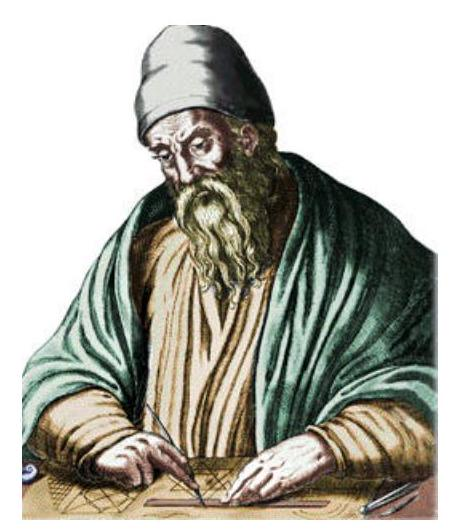
\includegraphics[max width=\textwidth, center]{2024_12_29_681ce8a6e73c53e2a13cg-04}
        Euclide
    \end{tcolorbox}
\end{minipage}

\subsection{Corollaires de l'algorithme d'Euclide}
\begin{proposition}{}{}
Pour tous $a, b \in \mathbb{N}^{*}$ et $d \in \mathbb{N}$ :

$$
d \mid a \text { et } d|b \Longleftrightarrow \hideM{d| \operatorname{PGCD}(a ; b)}
$$
\end{proposition}

\begin{demo}
Soient $a, b \in \mathbb{N}^{*}$.
Dans l'algorithme d'Euclide, $r_{0}$ est reste de la division euclidienne de $a$ par $b$. D'après démonstration de la propriété 1.2 , on sait que l'ensemble des diviseurs communs à $a$ et à $b$ est égale à l'ensemble des diviseurs communs à $b$ et à $r_{0}$. On note $E$ cet ensemble.\\
Comme $r_{1}$ est le reste de la division de $r_{0}$ par $b$, on en déduit que $E$ est aussi l'ensemble des diviseurs communs de $r_{0}$ et $r_{1}$.\\
En procédant par récurrence, on montre finalement que $E$ est l'ensemble des diviseurs communs de $r_{n_{0}-1}=\operatorname{PGCD}(a ; b)$ (le dernier reste non nul) et de 0 , ce qui correspond à l'ensemble des diviseurs de $\operatorname{PGCD}(a ; b)$.
\end{demo}

\begin{proposition}{}{}
Pour tous $a, b \in \mathbb{N}$ et $k \in \mathbb{N}$,

$$
\operatorname{PGCD}(k a ; k b)=\hideM{k \times \operatorname{PGCD}(a ; b)}
$$
\end{proposition}

\begin{demo}
Pour calculer $\operatorname{PGCD}(k a ; k b)$, toutes les étapes de l'algorithme d'Euclide seront les mêmes que pour calculer $\operatorname{PGCD}(a ; b)$ à un facteur multiplicatif $k$ près.
\end{demo}

\begin{definition}{}{}
Soient $a, b \in \mathbb{N}$ et $k \in \mathbb{Z}^{*}$.\\
On dit que $a$ et $b$ sont premiers entre eux lorsque $\hideM{\operatorname{PGCD}(a ; b)=1}$.
\end{definition}

\begin{proposition}{}{}
Soient $a, b \in \mathbb{N}^{*}$ et avec $d=\operatorname{PGCD}(a ; b)$.\\
Il existe des entiers premiers entre eux $a^{\prime}$ et $b^{\prime}$ tels que $\left\{\begin{array}{l}a=\hideM{d a^{\prime}} \\ b=\hideM{d b^{\prime}}\end{array}\right.$
\end{proposition}

\begin{demo}
Soient $a, b \in \mathbb{N}^{*}$ et $k \in \mathbb{Z}^{*}$ avec $d=\operatorname{PGCD}(a ; b)$. Comme $d$ est un diviseur commun de $a$ et $b$, il existe $a^{\prime}$ et $b^{\prime}$ des entiers tels que $a=d a^{\prime}$ et $b=d b^{\prime}$. Il suffit donc de montrer que $a^{\prime}$ et $b^{\prime}$ sont premiers entre eux. Or, on a :

$$
\begin{aligned}
\operatorname{PGCD}(a ; b) & =\operatorname{PGCD}\left(d a^{\prime} ; d b^{\prime}\right) \\
& =d \times \operatorname{PGCD}\left(a^{\prime} ; b^{\prime}\right)
\end{aligned}
$$

Ainsi, $d=d \times \operatorname{PGCD}\left(a^{\prime} ; b^{\prime}\right)$ et comme $d \neq 0$ ( $a$ et $b$ sont non nuls simultanément), on en déduit que $\operatorname{PGCD}\left(a^{\prime} ; b^{\prime}\right)=1$.
\end{demo}

\section{Identité et théorème de Bézout}
\subsection{Identité de Bézout}
\begin{proposition}{Identité de Bézout}{}
Soient $a, b \in \mathbb{N}^{*}$.\\
Il existe des entiers relatifs $u$ et $v$ tels que

$$
\hideM{a u+b v}=\operatorname{PGCD}(a ; b)
$$
\end{proposition}

\begin{demo}
On considère la suite des divisions de l'algorithme d'Euclide (où $r_{n_{0}-1}$ est le dernier reste non nul, c'est-à-dire $\left.r_{n_{0}-1}=\operatorname{PGCD}(a ; b)\right)$ :

$$
\begin{aligned}
& a=b q_{0}+r_{0} \\
& b=r_{0} q_{1}+r_{1} \\
& \vdots \\
& r_{k-1}=r_{k} q_{k+1}+r_{k+1} \\
& \vdots \\
& r_{n_{0}-4}= r_{n_{0}-3} q_{n_{0}-2}+r_{n_{0}-2}\\
& r_{n_{0}-3}= r_{n_{0}-2} q_{n_{0}-1}+r_{n_{0}-1} \\
& r_{n_{0}-2}=r_{n_{0}-1} q_{n_{0}}+0
\end{aligned}
$$

L'avant dernière égalité donne :


\begin{equation*}
\operatorname{PGCD}(a ; b)=r_{n_{0}-1}=r_{n_{0}-3}-r_{n_{0}-2} q_{n_{0}-1} \tag{$\star$}
\end{equation*}

Cela signifie que $\operatorname{PGCD}(a ; b)$ est une combinaison linéaire de $r_{n_{0}-3}$ et $r_{n_{0}-2}$. En exprimant $r_{n_{0}-2}$ dans la ligne du dessus et en la réinjectant dans l'égalité $\left({\star}\right)$, on obtient ensuite :

$$
\begin{aligned}
\operatorname{PGCD}(a ; b) & =r_{n_{0}-3}-\left(r_{n_{0}-4}-r_{n_{0}-3} q_{n_{0}-2}\right) q_{n_{0}-1} \\
& =r_{n_{0}-3}\left(1+q_{n_{0}-2}\right)-r_{n_{0}-4}
\end{aligned}
$$

Cela signifie que $\operatorname{PGCD}(a ; b)$ est une combinaison linéaire de $r_{n_{0}-4}$ et $r_{n_{0}-3}$. De proche en proche, on pourra finalement écrire $\operatorname{PGCD}(a ; b)$ comme une combinaison linéaire de $a$ et $b$.
\end{demo}

\begin{example}
On sait que $\operatorname{PGCD}(896 ; 259)=7$. Déterminer des entiers relatifs $u$ et $v$ tels que $896 u+259 v=7$. 
~\\Solution :\\
On écrit les différentes étapes de l'algorithme d'Euclide :

$$
\begin{aligned}
896 & =259 \times 3+119 \\
259 & =119 \times 2+21 \\
119 & =21 \times 5+14 \\
21 & =14 \times 1+7
\end{aligned}
$$

En remontant l'algorithme, on obtient:

$$
\begin{aligned}
7 & =21-14 \times 1 \\
& =21-(119-21 \times 5) \times 1 \\
& =6 \times 21-119 \\
& =6 \times(259-119 \times 2)-119 \\
& =6 \times 259-13 \times 119 \\
& =6 \times 259-13 \times(896-259 \times 3) \\
& =-13 \times 896+45 \times 259
\end{aligned}
$$

Ainsi, $896 u+259 v=7$ avec $u=-13$ et $v=45$.
\end{example}

\begin{method}{Déterminer une identité de Bézout avec deux entiers $a$ et $b$}{}
\begin{itemize}[noitemsep,topsep=0pt]
  \item Effectuer l'algorithme d'Euclide.
  \item Remonter les lignes de l'algorithme d'Euclide pour écrire $\operatorname{PGCD}(a ; b)$ comme une combinaison linéaire des restes jusqu'à obtenir une combinaison linéaire de $a$ et $b$.
\end{itemize}
\end{method}

\noindent
\begin{minipage}{.7\textwidth}
    \begin{history}{Identité de Bézout}{}
    L'identité de Bézout porte le nom du mathématicien français \textbf{Étienne Bézout} (1730-1783). Ce résultat avait cependant déjà été découvert et démontré par \textbf{Claude Gaspard Bachet de Méziriac} (1581-1638). Bézout a en fait généralisé un résultat similaire pour les polynômes. Pour cette raison, l'identité de Bézout prend parfois le nom de «théorème de Bachet-Bézout».
    \end{history}
\end{minipage}%
\hspace{1em}
\begin{minipage}{0.35\textwidth}
    \begin{tcolorbox}[colback=white,colframe=BrownHist]
        \centering
        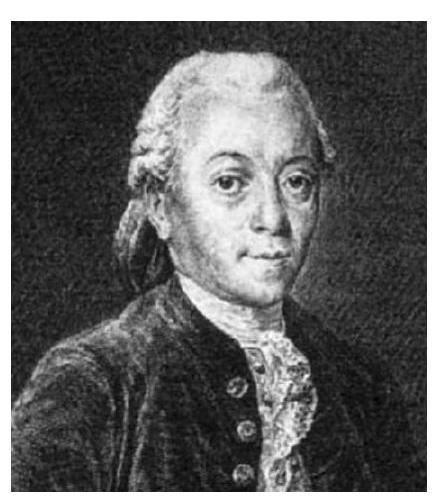
\includegraphics[max width=\textwidth, center]{2024_12_29_681ce8a6e73c53e2a13cg-06}
        Étienne Bézout
    \end{tcolorbox}
\end{minipage}

\subsection{Théorème de Bézout}
\begin{proposition}{Théorème de Bézout}{}
Soient $a, b \in \mathbb{Z}^{*}$. Les entiers $a$ et $b$ sont premiers entre eux si, et seulement si, il existe des entiers relatifs $u$ et $v$ tels que

$$
a u+b v=\hideM{1}
$$
\end{proposition}

\begin{proof}
\begin{itemize}[noitemsep,topsep=0pt]
  \item[]
  \item Supposons que $\operatorname{PGCD}(a ; b)=1$. D'après l'identité de Bézout, il est immédiat de voir qu'il existe des entiers relatifs $u$ et $v$ tels que $a u+b v=\operatorname{PGCD}(a ; b)=1$.
  \item Réciproquement, supposons qu'il existe des entiers relatifs $u$ et $v$ tels que $a u+b v=1$. Soit $d$ un diviseur commun de $a$ et $b$. On en déduit que $d$ divise la combinaison linéaire $a u+b v$ donc $d$ divise 1 . Ainsi, on en déduit que $d=1$ qui est le seul diviseur commun de $a$ et $b$.
  \\Par conséquent, $\operatorname{PGCD}(a ; b)=1$.
\end{itemize}
\end{proof}

\begin{remark}
\begin{itemize}[noitemsep,topsep=0pt]
  \item[]
  \item L'équivalence n'est vraie que si $\operatorname{PGCD}(a ; b)=1$.
  \\Dans le cas général, seule l'identité de Bézout est vraie.
  \item Le couple $(u ; v)$ de l'identité de Bézout n'est pas unique.
\end{itemize}
\end{remark}

\section{Théorème de Gauss et corollaire}
\subsection{Théorème de Gauss}
\begin{proposition}{Théorème de Gauss}{}
Soient $a, b, c \in \mathbb{Z}^{*}$.\\
Si $a \mid b c$ et si $a$ et $b$ sont premiers entre eux, alors $\hideM{a \mid c}$.
\end{proposition}

\begin{demo}
Soient $a, b, c \in \mathbb{Z}^{*}$ tels que $a \mid b c$ et tels que $a$ et $b$ sont premiers entre eux.\\
$a$ et $b$ sont premiers entre eux donc, d'après le théorème de Bézout, il existe des entiers $u$ et $v$ tels que $a u+b v=1$. Ainsi, en multipliant par $c$, on obtient :

$$
a u c+b v c=c
$$

Comme $a \mid a$ et $a \mid b c$, on en déduit que $a$ divise la combinaison linéaire $a u c+b c v$, c'est-à-dire $a \mid c$.
\end{demo}

\begin{remark}
La condition « $a$ et $b$ sont premiers entre eux» est indispensable.\\
En effet, 9 divise $6 \times 15=90$ et pourtant 9 ne divise ni 6 , ni 15 .
\end{remark}

\noindent
\begin{minipage}{.7\textwidth}
    \begin{history}{Théorème de Gauss}{}
    \textbf{Carl Friedrich Gauß} (1777-1855) est l'un des mathématiciens les plus célèbres du XIXe siècle. On le surnomme «le prince des mathématiques » et il existe un nombre important de résultats qui portent son nom. Il a démontré le théorème ci-dessus en 1801 dans un ouvrage intitulé Diquisitiones arithmeticae. C'est d'ailleurs la même année qu'il a déterminé la trajectoire de la planète naine Cérès en utilisant notamment la méthode des moindres carrés.
    \end{history}
\end{minipage}%
\hspace{1em}
\begin{minipage}{0.35\textwidth}
    \begin{tcolorbox}[colback=white,colframe=BrownHist]
        \centering
        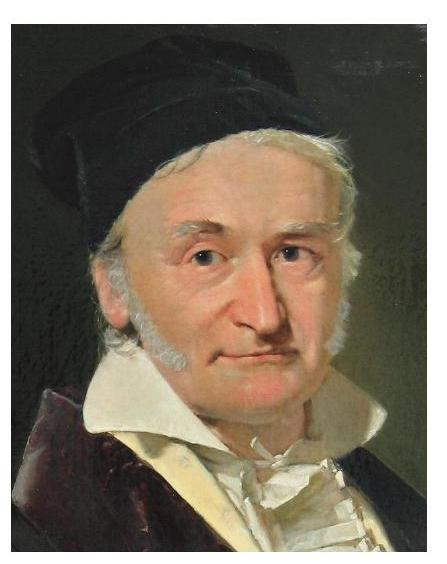
\includegraphics[max width=\textwidth, center]{2024_12_29_681ce8a6e73c53e2a13cg-08}
        Carl Friedrich Gauß
    \end{tcolorbox}
\end{minipage}

\subsection{Corollaire du théorème de Gauss}
\begin{proposition}{(Corollaire)}{}
Soient $a, b, c \in \mathbb{Z}^{*}$ tels que $b|a, c| a$ et tels que $\operatorname{PGCD}(b ; c)=1$, alors $\hideM{b c \mid a}$.
\end{proposition}

\begin{demo}
Soient $a, b, c \in \mathbb{Z}^{*}$ tels que $b|a, c| a$ et tels que $\operatorname{PGCD}(b ; c)=1$.\\
Comme $b \mid a$ et $c \mid a$, il existe des entiers $k$ et $l$ tels que $a=b k=c l$. Ainsi, $c \mid b k$.\\
Mais comme $b$ et $c$ sont premiers entre eux, on en déduit d'après le théorème de Gauss que $c \mid k$.\\
Donc il existe un entier $k^{\prime}$ tel que $k=c k^{\prime}$.\\
Finalement, on obtient $a=b\left(c k^{\prime}\right)=b c k^{\prime}$ donc $b c \mid a$.\\
\end{demo}

La propriété précédente se reformule à l'aide de congruences de la façon suivante :

\begin{proposition}{(Corollaire)}{}
Soient $a, b, c \in \mathbb{Z}^{*}$.

$$
\left\{
\begin{array}{rl}
& a \equiv \hideM{0}[b] \\
& a \equiv \hideM{0}[c] \\
& \operatorname{PGCD}(b ; c)=\hideM{1}
\end{array} \Longrightarrow a \equiv \hideM{0}[b c] .
\right.
$$
\end{proposition}

\newpage
\section{Applications}
\subsection{Études de divisibilité}
\begin{example}
Soit $p \geqslant 5$ un nombre premier. Montrer que $p^{2}-1$ est divisible par 24.\\
~\\Solution :\\
Comme $24=8 \times 3$, on commence par montrer que $p^{2}-1$ est divisible par 8 et par 3 .

\begin{itemize}[noitemsep,topsep=0pt]
  \item En raisonnant modulo 8 (on sait que $p$ est impair) :

\begin{center}
\begin{tabular}{|c|c|c|c|c|c|c|c|c|}
\hline
$p[8]$ & 0 & 1 & 2 & 3 & 4 & 5 & 6 & 7 \\
\hline
$p^{2}-1[8]$ & $\times$ & 0 & $\times$ & 0 & $\times$ & 0 & $\times$ & 0 \\
\hline
\end{tabular}
\end{center}

Ainsi, cela prouve que pour tout $p \geqslant 5$ premier, $8 \mid p^{2}-1$.

  \item En raisonnant modulo 3 :

\begin{center}
\begin{tabular}{|c|c|c|c|}
\hline
$p[3]$ & 0 & 1 & 2 \\
\hline
$p^{2}-1[3]$ & $\times$ & 0 & 0 \\
\hline
\end{tabular}
\end{center}

Ainsi, cela prouve que pour tout $p \geqslant 5,3 \mid p^{2}-1$.

  \item Finalement, on a prouvé que pour tout nombre premier $p \geqslant 5,3 \mid p^{2}-1$ et $8 \mid p^{2}-1$. D'après le théorème de Gauss (son corollaire), comme $\operatorname{PGCD}(8 ; 3)=1$, on en déduit que $24 \mid p^{2}-1$.
\end{itemize}
\end{example}

\begin{method}{Établir une relation de divisibilité par $n$}{}
\begin{itemize}[noitemsep,topsep=0pt]
  \item Décomposer $n$ comme un produit de facteurs premiers entre eux.
  \item Montrer que la quantité considérée est divisible par chacun des facteurs.
  \item Utiliser le théorème de Gauss (corollaire).
\end{itemize}
\end{method}

\subsection{Démonstration de l'irrationalité de $\sqrt{2}$}

\noindent
\begin{minipage}{.7\textwidth}
    \begin{history}{Crise des irrationnels}{}
    La découverte de l'irrationalité de $\sqrt{2}$ a provoqué une véritable crise dans les mathématiques grecques. À l'époque, les mathématiciens considéraient en effet que le monde physique peut se comprendre à travers des rapports de longueurs entières. Une légende dit même que le mathématicien \textbf{Hippase de Métaponte} (500 av. J.-C.) qui a découvert le caractère « incommensurable» (irrationnel) de $\sqrt{2}$ a été condamné à la noyade par ses condisciples. Si cela n'est pas du tout assuré historiquement, il n'en reste pas moins que cette histoire traduit les difficultés qu'ont eu les grecs à accepter l'existence de nombres irrationnels.
    \end{history}
\end{minipage}%
\hspace{1em}
\begin{minipage}{0.35\textwidth}
    \begin{tcolorbox}[colback=white,colframe=BrownHist]
        \centering
        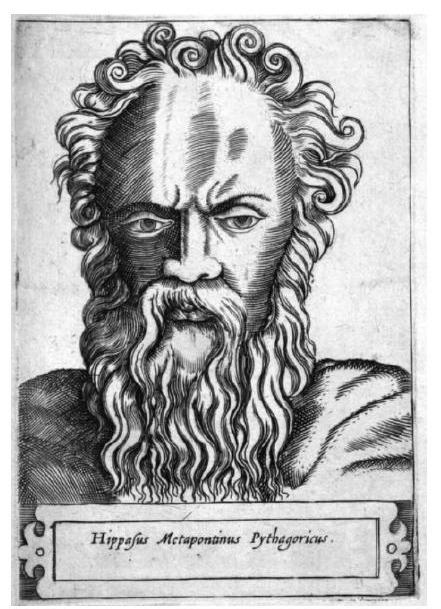
\includegraphics[max width=\textwidth, center]{2024_12_29_681ce8a6e73c53e2a13cg-09}
        Hippase de Métaponte
    \end{tcolorbox}
\end{minipage}

\begin{proposition}{(Lemme)}{}
Soit $a \in \mathbb{Z}$. Alors,

\begin{itemize}[noitemsep,topsep=0pt]
  \item $a$ est pair $\Longleftrightarrow a^{2}$ est \hide{pair}.
  \item $a$ est impair $\Longleftrightarrow a^{2}$ est \hide{impair}.
\end{itemize}
\end{proposition}

\begin{demo}
Soit $a \in \mathbb{Z}$.

\begin{itemize}[noitemsep,topsep=0pt]
  \item On suppose que $a$ est pair.

Il existe $k \in \mathbb{Z}$ tel que $a=2 k$.\\
Donc $a^{2}=(2 k)^{2}=4 k^{2}=2 \times 2 k^{2}$.\\
On pose $k^{\prime}=2 k^{2}$.\\
On a donc $a^{2}=2 k^{\prime}$, ce qui signifie que $a^{2}$ est pair.

  \item On suppose que $a$ est impair.

Il existe $k \in \mathbb{Z}$ tel que $a=2 k+1$.\\
Donc $a^{2}=(2 k+1)^{2}=4 k^{2}+4 k+1=2 \times\left(2 k^{2}+2 k\right)+1$.\\
On pose $k^{\prime}=2 k^{2}+2 k$.\\
On a donc $a^{2}=2 k^{\prime}+1$, ce qui signifie que $a^{2}$ est impair.

  \item On suppose que $a^{2}$ est pair.

On souhaite montrer que $a$ est nécessairement pair.\\
En fait, si $a$ était impair, on a montré que $a^{2}$ serait impair, ce qui serait absurde.

  \item On raisonne de même pour montrer que si $a^{2}$ est impair, alors $a$ est impair.
\end{itemize}
\end{demo}

\begin{proposition}{}{}
Le nombre réel $\sqrt{2}$ est \hide{irrationnel}.
\end{proposition}

\begin{demo}
On suppose par l'absurde qu'il existe deux entiers $a$ et $b$ premiers entre eux (avec $b \neq 0$ ) tels que $\sqrt{2}=\dfrac{a}{b}$.\\
Ainsi, en élevant cette égalité au carré, on obtient :

$$
2=\frac{a^{2}}{b^{2}}
$$

Donc $a^{2}=2 b^{2} \quad\left({ }^{*}\right)$\\
Cela signifie que $a^{2}$ est pair et donc que $a$ est pair d'après le lemme précédent (propriété 4.2). Ainsi, il existe $k \in \mathbb{Z}$ tel que $a=2 k$.\\
En réinjectant dans l'égalité $\left({ }^{*}\right)$, on obtient : $4 k^{2}=2 b^{2}$ donc $2 k^{2}=b^{2}$.\\
Cela signifie que $b^{2}$ est pair et donc que $b$ est pair d'après le lemme précédent.\\
Finalement, $a$ et $b$ sont tous les deux pairs, ce qui est absurde car ils ont été supposés premiers entre eux.
\end{demo}

\subsection{Détermination d'un inverse modulo $n$}
\begin{proposition}{}{}
Soint $n \geqslant 2$. Alors $a \in \mathbb{N}$ est inversible modulo $n$ si, et seulement si, $\hideM{\operatorname{PGCD}(a ; n)=1}$.
\end{proposition}

\begin{demo}
Soit $n \geqslant 2$ et $a \in \mathbb{N}$. Alors,\\
$\operatorname{PGCD}(a ; n)=1$\\
$\Longleftrightarrow$ il existe $u, v \in \mathbb{Z}$ tels que $a u+n v=1$\\
$\Longleftrightarrow$ il existe $u, v \in \mathbb{Z}$ tels que $1-a u=n v$\\
$\Longleftrightarrow$ il existe $u \in \mathbb{Z}$ tel que $n \mid 1-a u$\\
$\Longleftrightarrow$ il existe $u \in \mathbb{Z}$ tel que $1-a u \equiv 0[n]$\\
$\Longleftrightarrow$ il existe $u \in \mathbb{Z}$ tel que $a u \equiv 1[n]$.
\end{demo}

\begin{example}
Montrer que 13 est inversible modulo 36 et déterminer son inverse.

~\\Solution :\\
On effectue l'algorithme d'Euclide :

$$
\begin{aligned}
& 36=13 \times 2+10 \\
& 13=10 \times 1+3 \\
& 10=3 \times 3+1
\end{aligned}
$$

Ainsi, $\operatorname{PGCD}(13 ; 36)=1$ donc 13 est bien inversible modulo 36.\\
Par ailleurs, en remontant l'algorithme d'Euclide :

$$
\begin{aligned}
1 & =10-3 \times 3 \\
& =10-(13-10 \times 1) \times 3 \\
& =4 \times 10-3 \times 13 \\
& =4 \times(36-13 \times 2)-3 \times 13 \\
& =4 \times 36-11 \times 13
\end{aligned}
$$

Ainsi, en considérant la dernière égalité modulo 36, on voit que $-11 \times 13=1$ [36].\\
Cela signifie donc que l'inverse de 13 est -11 , soit 25 modulo 36 .
\end{example}

\begin{method}{Déterminer l'inverse de $a$ modulo $n$}{}
\begin{itemize}[noitemsep,topsep=0pt]
  \item Déterminer une identité de Bézout entre $a$ et $n$ :
\end{itemize}

$$
a u+n v=1
$$

\begin{itemize}[noitemsep,topsep=0pt]
  \item Considérer l'égalité modulo $n$.
\end{itemize}
\end{method}

\newpage

\subsection{Résolution d'équations diophantiennes}
On appelle équation diophantienne une équation à coefficients entiers pour laquelle on cherche les solutions entières.

\noindent
\begin{minipage}{.7\textwidth}
    \begin{history}{Crise des irrationnels}{}
    Mathématicien grec de l'antiquité, \textbf{Diophante} est l'auteur d'Arithmetica dans lequel il résout certaines équations où les inconnues sont des entiers. Par la suite, de nombreux mathématiciens se sont intéressés à ce genre d'équations. En général, l'équation posée correspond à un problème facilement compréhensible mais qui peut être très difficile à résoudre. Á noter que la plupart du temps, les équations diophantiennes n'ont pas d'application immédiate, en physique par exemple. Elles ont cependant poussé les mathématiciens à développer de nouvelles théories au cours de l'histoire. L'exemple du grand théorème de Fermat qui a été conjecturé par \textbf{Pierre de Fermat} au XVIIe siècle et démontré plus de trois siècles plus tard par \textbf{Andrew Wiles} en 1994 en est un exemple frappant. Ce théorème énonce que pour tout $n \geqslant 3$, il n'existe pas de triplet d'entiers non nuls $(x ; y ; z)$ tels que $x^{n}+y^{n}=z^{n}$.
    \end{history}
\end{minipage}%
\hspace{1em}
\begin{minipage}{0.35\textwidth}
    \begin{tcolorbox}[colback=white,colframe=BrownHist]
        \centering
        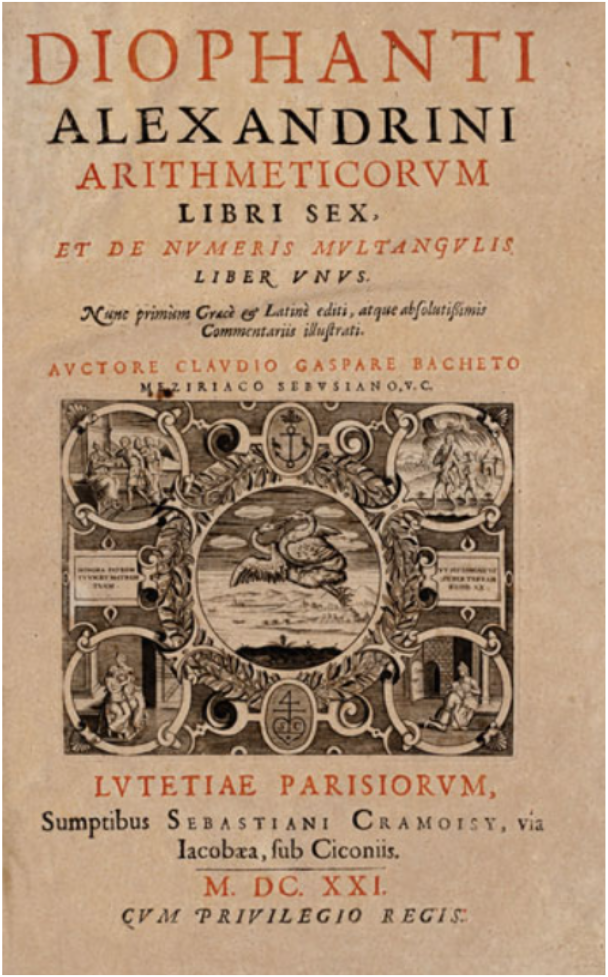
\includegraphics[max width=\textwidth, center]{swappy-20241229_193230.png}
        Édition de 1621 de Arithmetica
    \end{tcolorbox}
\end{minipage}

\subsubsection{Résolution d'équations de la forme $a x=b y$}
\begin{example}
Résoudre dans $\mathbb{Z}^{2}$ l'équation (E) : $36 x=45 y$.\\
~\\Solution :\\
On a $\operatorname{PGCD}(36 ; 45)=9$.\\
On simplifie par l'équation en divisant par 9 :

$$
36 x=45 y \Longleftrightarrow 4 x=5 y
$$

Analyse : Supposons que $(x ; y)$ est une solution de l'équation (E).\\
Alors $4 x=5 y$ donc, d'après le théorème de Gauss, comme 4 et 5 sont premiers entre eux, on en déduit que $4 \mid y$.\\
Ainsi, il existe $k \in \mathbb{Z}$ tel que $y=4 k$.\\
Par la suite, on en déduit que $4 x=5 \times(4 k)$ et donc que $x=5 k$.\\
Synthèse : Pour tout $k \in \mathbb{Z}$, le couple ( $5 k ; 4 k$ ) est une solution de (E).\\
Finalement, on a montré que $\mathcal{S}=\{(5 k ; 4 k), k \in \mathbb{Z}\}$.
\end{example}

\begin{method}{Résoudre une équation de la forme $a x=b y$}{}
\begin{itemize}[noitemsep,topsep=0pt]
  \item Simplifier en divisant l'équation par $\operatorname{PGCD}(a ; b)$
  \item Procéder par analyse / synthèse en utilisant le théorème de Gauss.
\end{itemize}
\end{method}

\subsubsection{Résolution d'équations de la forme $a x+b y=k$}
\begin{proposition}{}{}
Soient $a, b \in \mathbb{Z}^{*}$ et $k \in \mathbb{Z}^{*}$.\\
L'équation $a x+b y=k$ (d'inconnues $x$ et $y$ ) admet des solutions entières si, et seulement si, $\hideM{\operatorname{PGCD}(a ; b) \mid k}$.
\end{proposition}

\begin{demo}
\begin{itemize}[noitemsep,topsep=0pt]
  \item Supposons que l'équation $a x+b y=k$ admette une solution. Cela signifie qu'il existe des entiers $x_{0}$ et $y_{0}$ tels que $a x_{0}+b y_{0}=k$. Comme $\operatorname{PGCD}(a ; b)$ est un diviseur commun de $a$ et $b$, il divise toute combinaison linéaire de $a$ et $b$. En particulier, $\operatorname{PGCD}(a ; b)$ divise $a x_{0}+b y_{0}=k$.
  \item Réciproquement, supposons que $\operatorname{PGCD}(a ; b) \mid k$. Cela signifie qu'il existe $k^{\prime} \in \mathbb{Z}$ tel que $k=\operatorname{PGCD}(a ; b) \times k^{\prime}$. Or, d'après l'identité de Bézout, il existe des entiers $u_{0}$ et $v_{0}$ tels que $a u_{0}+b v_{0}=\operatorname{PGCD}(a ; b)$. En multipliant cette égalité par $k^{\prime}$, il vient :
  $$
  a u_{0} k^{\prime}+b v_{0} k^{\prime}=\operatorname{PGCD}(a ; b) \times k^{\prime}
  $$
  On pose $x_{0}=u_{0} k^{\prime}$ et $y_{0}=v_{0} k^{\prime}$. Il est alors clair que le couple $\left(x_{0} ; y_{0}\right)$ est solution de l'équation $a x+b y=k$.
\end{itemize}
\end{demo}

\begin{example}
Déterminer l'ensemble des couples solutions des équations suivantes :

\begin{enumerate}[noitemsep,topsep=0pt]
  \item $15 x+33 y=7$
  \item $14 x+32 y=8$.
\end{enumerate}

~\\Solution :\\
\begin{enumerate}
  \item $\operatorname{PGCD}(15,33)=3$. Comme 3 ne divise pas 7 , l'équation n'admet aucune solution.\\
  En effet, si $(x ; y)$ était un couple solution, on aurait $15 x+33 y=7$. Comme 3 divise 15 et 33 , il faudrait qu'il divise 7 , ce qui n'est pas le cas.
  \item On détermine le PGCD de 14 et 32 avec l'algorithme d'Euclide.
$$
\begin{aligned}
32 & =14 \times 2+4 \\
14 & =4 \times 3+2 \\
4 & =2 \times 2+0
\end{aligned}
$$
Ainsi, $\operatorname{PGCD}(14 ; 32)=2$ et comme 2 divise 8 l'équation admet des solutions. En remontant l'algorithme d'Euclide, il vient :
$$
\begin{aligned}
2 & =14-4 \times 3 \\
& =14-(32-14 \times 2) \times 3 \\
& =-3 \times 32+7 \times 14
\end{aligned}
$$
Ainsi, en multipliant la dernière égalité par 4, il vient
$$
8=-12 \times 32+28 \times 14
$$
En posant, $x_{0}=28$ et $y_{0}=-12$, on voit que le couple $\left(x_{0} ; y_{0}\right)$ est une solution de l'équation. Soit $(x, y) \in\left(\mathbb{Z}^{*}\right)^{2}$ :
$$
\begin{aligned}
14 x+32 y=8 & \Longleftrightarrow 14 x+32 y=14 x_{0}+32 y_{0} \\
& \Longleftrightarrow 14\left(x-x_{0}\right)=32\left(y_{0}-y\right) \\
& \Longleftrightarrow 7\left(x-x_{0}\right)=16\left(y_{0}-y\right)
\end{aligned}
$$
Analyse : Supposons que $x$ et $y$ sont solutions.\\
Alors, d'après le théorème de Gauss, $7 \mid y_{0}-y($ car $\operatorname{PGCD}(7 ; 16)=1)$.\\
Donc il existe $k \in \mathbb{Z}$ tel que $y_{0}-y=7 k$, c'est-à-dire $y=y_{0}-7 k=-12-7 k$.\\
En réinjectant cette expression dans l'égalité (*), on obtient : $7\left(x-x_{0}\right)=16 \times 7 k$.\\
Ainsi, $x-x_{0}=16 k$, c'est-à-dire $x=x_{0}+16 k=28+16 k$.

~\\Synthèse : Si on pose $x=28+16 k$ et $y=-12-7 k$ (avec $k \in \mathbb{Z}$ ), il est immédiat de vérifier que le couple $(x ; y)$ est bien une solution de l'équation.

~\\Finalement, $\mathcal{S}=\{(28+16 k ;-12-7 k), k \in \mathbb{Z}\}$
\end{enumerate}
\end{example}

\begin{method}{Résoudre une équation diophantienne de la forme $a x+b y=k$}{}
\begin{itemize}[noitemsep,topsep=0pt]
  \item Effectuer l'algorithme d'Euclide pour déterminer $\operatorname{PGCD}(a ; b)$
  \item Remonter l'algorithme afin de trouver une solution particulière $\left(x_{0} ; y_{0}\right)$.
  \item Ecrire qu'un couple $(x ; y)$ est solution $\Longleftrightarrow a x+b y=a x_{0}+b y_{0}$.
  \item Passer les x du même côté et les y du même côté puis conclure avec Gauss.
\end{itemize}
\end{method}

\vspace{1em}

\begin{savoir}{}{}
\begin{itemize}[noitemsep,topsep=0pt]
  \item Déterminer le PGCD de deux entiers avec l'algorithme d'Euclide.
  \item Déterminer une relation de Bézout entre deux entiers.
  \item Connaître et utiliser les théorèmes de Bézout et de Gauss.
  \item Étudier une relation de divisibilité.
  \item Démontrer l'irrationalité de $\sqrt{2}$.
  \item Déterminer un inverse modulo $n$.
  \item Résoudre des équations diophantiennes de la forme $a x=$ by.
  \item Résoudre des équations diophantiennes de la forme $a x + by = k$.
\end{itemize}
\end{savoir}

\end{document}